% ToonSense -- 8-page IEEE conference version.
% Extended version (all detail tables in an appendix): main_extended.tex. Supplementary material: supplementary.tex.
\documentclass[conference]{IEEEtran}
\usepackage[utf8]{inputenc}
\usepackage[T1]{fontenc}
\usepackage{graphicx}
\usepackage{booktabs}
\usepackage{adjustbox}
\usepackage{amsmath,amssymb}
\usepackage{multirow}
\usepackage{url}
\usepackage[hidelinks]{hyperref}

\title{ToonSense: Robust Multimodal Understanding of Cartoon-Driven Bangla--English Code-Mixed Memes}
\author{\IEEEauthorblockN{Adrita Biswas, Atanu Dewanjee, Hrittika Dutta}
\IEEEauthorblockA{School of Science, Engineering and Technology\\
East Delta University, Chattogram, Bangladesh}}

\begin{document}
\maketitle

\begin{abstract}
Multimodal meme classifiers are evaluated on clean benchmarks, yet memes circulate in Romanised spellings, with mixed
languages and degraded images. We present ToonSense, a robustness study of frozen-encoder multimodal models for
Bangla--English memes, centred on cartoon memes from CMBan and replicated on BanglaAbuseMeme and MemoSen. We benchmark
six multilingual text encoders, four image encoders and five fusion heads with repeated cross-validation and
Holm-corrected tests, subject XLM-R + CLIP ViT-B/32 models to twelve linguistic and visual perturbations at three
severities, compare Integrated Gradients and Grad-CAM attributions before and after perturbation, and categorise
errors. Image features carry most of the signal, and fusion adds a small but significant gain on the larger datasets.
Romanised Bangla is the most damaging perturbation on every dataset, reducing fusion macro-F1 by 8--21\% relative,
whereas native-script spelling noise and code-mixing are nearly harmless. The perturbed text gains rather than loses
attribution share, and visual perturbations flip up to 27\% of predictions with small F1 changes. Training-time
augmentation with transliterated copies cuts the Romanisation drop to 2--5\%, including for an unseen spelling style,
at a clean-accuracy cost below one point.
\end{abstract}

\begin{IEEEkeywords}
Bangla memes, multimodal classification, code-mixing, robustness, Romanisation, CLIP, XLM-R, explainability
\end{IEEEkeywords}

\section{Introduction}
\label{sec:intro}

Internet memes combine an image with overlaid text, and their meaning usually arises from the interaction of the two:
a harmless caption becomes sarcastic or offensive in front of a particular picture. This has motivated multimodal
datasets and models for meme sentiment, humour, offensiveness and hate~\cite{kiela2020hateful,sharma2020memotion}.
Bangla, spoken by more than 250 million people, now has dedicated meme
resources~\cite{hossain2022memosen,hossain2022mute,das2023banglaabusememe,hossain2024bhm}. The most recent,
CMBan~\cite{cmban2025}, targets \emph{cartoon-driven} memes written in Bangla, English or a mix of both.

All of these works evaluate on held-out \emph{clean} data. Memes on social media are not clean. The same joke
circulates in Bangla script and in Romanised ``Banglish'' with inconsistent spelling, English insertions and added or
stripped emojis, and the image is recompressed, cropped and resized as it is shared. A model that scores well on a
benchmark may fail on these variants. To our knowledge, no prior work measures how Bangla meme classifiers behave
under such variation.

We present \textbf{ToonSense}, a robustness study of frozen-encoder multimodal classifiers on Bangla--English memes.
It asks (Q1) how much text, image and fusion contribute to clean accuracy, (Q2) how much accuracy drops under
realistic linguistic and visual perturbations, and (Q3) why the models fail. Our contributions are:
\begin{itemize}
  \item \textbf{A robustness framework for Bangla memes} with twelve perturbation families at three severities,
  including a colloquial Bangla-to-Banglish transliterator and OCR-guided text occlusion, evaluated by the Robustness
  Drop and the label-free flip rate.
  \item \textbf{A multi-encoder benchmark} of six frozen text encoders, four image encoders and five fusion heads
  with repeated cross-validation and Holm-corrected tests, on the public CMBan subset and replicated on
  BanglaAbuseMeme~\cite{das2023banglaabusememe} and MemoSen~\cite{hossain2022memosen}.
  \item \textbf{Comparative explainability and an error taxonomy}: attribution shifts before and after perturbation
  (Integrated Gradients, Grad-CAM) and a source attribution of errors.
  \item \textbf{A mitigation}: train-time Romanisation augmentation that needs no new labels.
\end{itemize}
The main findings are that image features carry most of the signal; that Romanised Bangla is the most damaging
perturbation on every dataset (8--21\% relative macro-F1 loss for fusion) while native-script spelling noise is
nearly harmless; that the perturbed text \emph{gains} attribution share; and that transliteration augmentation removes
most of the drop at a clean cost below one point.

\section{Related Work}
\label{sec:related}

\textbf{Meme understanding.} The Hateful Memes challenge~\cite{kiela2020hateful} showed that unimodal models fail when
either modality alone is benign, and Memotion~\cite{sharma2020memotion} introduced the humour, sarcasm, offensiveness,
motivation and sentiment taxonomy that CMBan adopts. Most systems fuse a pretrained text encoder with a vision
encoder, often CLIP~\cite{radford2021clip}. Bangla resources include MemoSen~\cite{hossain2022memosen} (sentiment),
MUTE~\cite{hossain2022mute} and BHM~\cite{hossain2024bhm} (hate), BanglaAbuseMeme~\cite{das2023banglaabusememe}
(abuse, vulgarity, sarcasm, sentiment), MIMOSA~\cite{ahsan2024mimosa} (aggression) and CMBan~\cite{cmban2025}, which
annotates 2{,}641 cartoon memes along the Memotion dimensions. All evaluate on clean data only.

\textbf{Robustness.} ImageNet-C~\cite{hendrycks2019benchmarking} established severity-graded corruptions for vision,
CheckList~\cite{ribeiro2020checklist} behavioural testing for NLP, and GLUECoS~\cite{khanuja2020gluecos} showed that
multilingual encoders degrade on code-switched input. CLIP reads rendered text and is therefore susceptible to
typographic manipulation~\cite{goh2021multimodal}, which matters for memes, where the text \emph{is} part of the
image. For Bangla, the dominant real-world variation is Romanised writing, which has not been studied for memes.

\textbf{Explainability.} Integrated Gradients~\cite{sundararajan2017ig} and
Grad-CAM~\cite{selvaraju2017gradcam,chattopadhay2018gradcampp} are widely used to justify predictions. We use them
\emph{comparatively}, measuring how modality reliance and visual attention shift between clean and perturbed versions
of the same meme.

\section{Methodology}
\label{sec:method}

Fig.~\ref{fig:flow} summarises ToonSense. Text and image are encoded by frozen pretrained encoders, and a lightweight
head is trained on the cached embeddings for each task. Perturbations are injected \emph{before} the encoders, so the
same trained heads are evaluated on clean and perturbed versions of the same memes. Freezing the encoders keeps the
study affordable and ensures that a perturbation changes only the input, never the evaluated classifier.

\begin{figure*}[t]
  \centering
  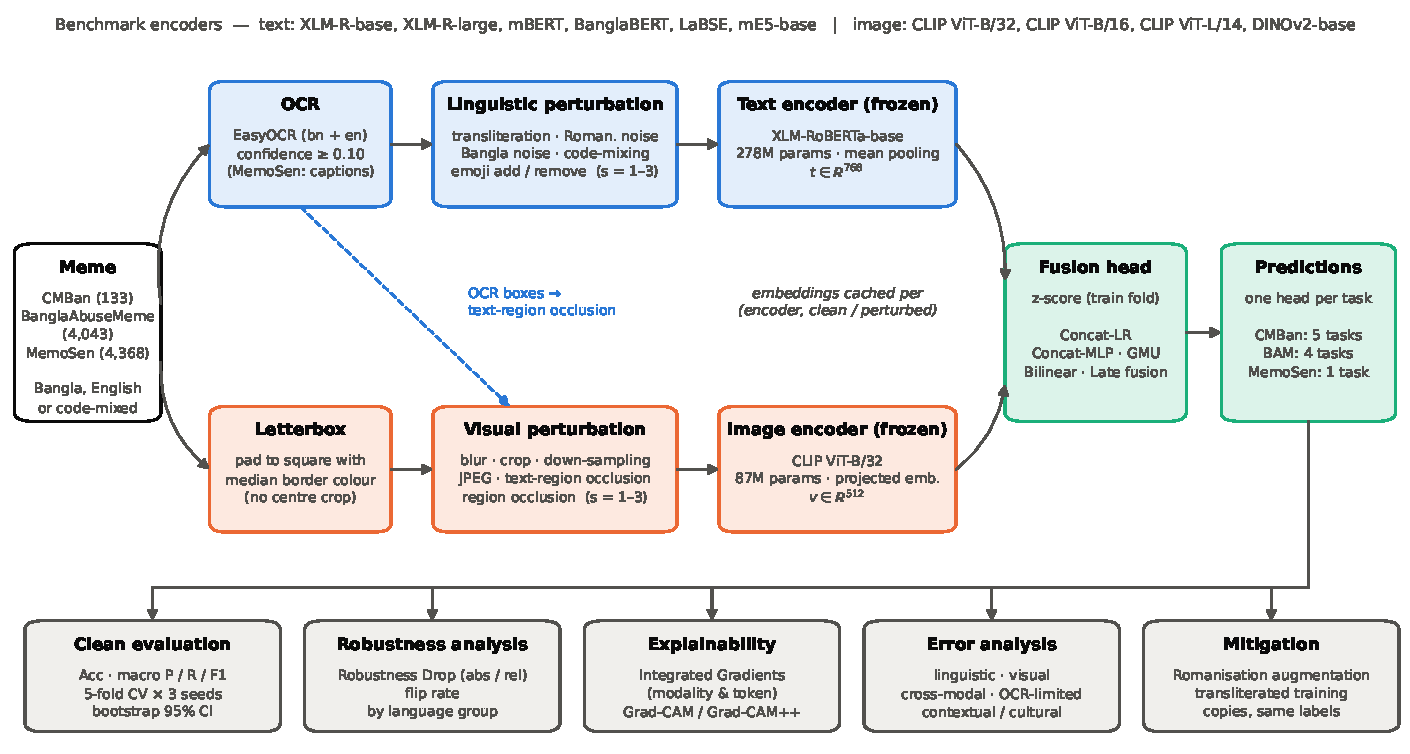
\includegraphics[width=\textwidth]{figures/methodology_flow.pdf}
  \caption{ToonSense pipeline. Meme text comes from OCR (MemoSen: human captions) and is encoded by XLM-R-base; the
  letterboxed image is encoded by CLIP ViT-B/32. Linguistic and visual perturbations ($s\in\{1,2,3\}$) are applied
  before the frozen encoders. Predictions feed the clean, robustness, explainability and error analyses, and a
  train-time augmentation tests a mitigation. Alternative encoders (top) are used in the benchmark.}
  \label{fig:flow}
\end{figure*}

\subsection{Datasets}
\label{sec:method:data}

Table~\ref{tab:datasets} lists the three datasets, which are processed \emph{separately}; only the protocol is
shared. CMBan~\cite{cmban2025} reports 2{,}641 memes, but labels are public for only 133 (85 Bangla, 45 code-mixed,
3 English). Because several fine classes are tiny, we use coarse labels that collapse intensity levels (e.g.\ funny
vs.\ not funny). To test whether findings hold at scale, we repeat the full protocol on
BanglaAbuseMeme~\cite{das2023banglaabusememe} (BAM), whose text is rendered in the image, and
MemoSen~\cite{hossain2022memosen}, which ships human-written captions and so removes OCR noise. Memes are grouped by
script as Bangla ($\geq$85\% Bangla letters), Latin-script ($\leq$15\%) or code-mixed.

\begin{table}[t]
\centering
\small
\caption{Datasets. Classes in parentheses (CMBan: fine/coarse).}
\label{tab:datasets}
\begin{adjustbox}{max width=\columnwidth}
\begin{tabular}{lrll}
\toprule
Dataset & $N$ & Tasks (classes) & Text \\
\midrule
CMBan & 133 & humour, sarcasm, offensive (3/2), & OCR \\
 & & motivational (2), sentiment (5/3) & \\
BAM & 4{,}043 & sentiment (3), sarcasm, abuse, vulgarity (2) & OCR \\
MemoSen & 4{,}368 & sentiment (3) & human \\
\bottomrule
\end{tabular}
\end{adjustbox}
\end{table}

\subsection{Encoders and Heads}
\label{sec:method:enc}

\textbf{Pre-processing.} Text is extracted with EasyOCR~\cite{easyocr} (Bangla+English); fragments with confidence
below 0.10 are dropped and the rest ordered in reading order. Mean OCR confidence is 0.58 (CMBan) and 0.54 (BAM).
Images are letterboxed to a square before encoding, so tall multi-panel comics are not cropped.

\textbf{Encoders.} The primary pair is XLM-RoBERTa-base~\cite{conneau2020xlmr} (mean-pooled, 768-d) and CLIP
ViT-B/32~\cite{radford2021clip} (512-d projection). For the benchmark we add XLM-R-large, mBERT~\cite{devlin2019bert},
BanglaBERT~\cite{bhattacharjee2022banglabert}, LaBSE~\cite{feng2022labse} and mE5-base~\cite{wang2024me5} as text
encoders, and CLIP ViT-B/16, ViT-L/14 and DINOv2-base~\cite{oquab2024dinov2} as image encoders. We chose the primary
pair for its coverage of Bangla, English and Romanised tokens in one vocabulary, its language-supervised image
features and its cost: CLIP-B/32 is the smallest image encoder, which matters because the robustness protocol
re-encodes 36 perturbed copies of every dataset.

\textbf{Heads.} Embeddings are standardised per training fold. Unimodal heads are an $\ell_2$-regularised logistic
regression (LR) and a two-layer MLP ($H=256$, GELU, dropout 0.3). Fusion heads are \emph{Concat-LR/MLP} on
$[\mathbf{t};\mathbf{v}]$; a \emph{GMU}~\cite{arevalo2017gmu},
$\mathbf{h}=\mathbf{z}\odot\tanh(W_t\mathbf{t})+(1-\mathbf{z})\odot\tanh(W_v\mathbf{v})$ with
$\mathbf{z}=\sigma(W_z[\mathbf{t};\mathbf{v}])$; a \emph{bilinear} head on
$[\mathbf{a};\mathbf{b};\mathbf{a}\odot\mathbf{b};|\mathbf{a}-\mathbf{b}|]$ of projected embeddings; and \emph{late
fusion}, averaging text- and image-MLP probabilities. Baselines are the majority class and a character 2--5-gram
TF-IDF + LR. Neural heads use AdamW ($10^{-3}$), class-weighted cross-entropy and early stopping (patience 30) on an
inner validation split, on which the LR regularisation $C\in\{0.01,0.1,1\}$ is also selected.

\subsection{Perturbations}
\label{sec:method:pert}

Table~\ref{tab:perturbations} lists six linguistic and six visual families. \emph{Transliteration} uses a rule-based
Bangla-to-Banglish converter written for this study that follows colloquial conventions (schwa deletion,
\textit{ya-}/\textit{ba-phala}); \emph{Romanised spelling noise} romanises fully and then applies common Banglish
variants (\textit{sh}$\leftrightarrow$\textit{s}, \textit{bh}$\to$\textit{v}, vowel dropping); \emph{Bangla spelling
noise} swaps confusable native characters; \emph{code-mixing} switches words with a $\sim$200-word bilingual lexicon.
\emph{Text occlusion} fills OCR boxes with their median colour, and \emph{region occlusion} greys out non-text grid
cells. Perturbations are deterministic per meme, family and severity. A linguistic perturbation changes only the text
input and a visual one only the image input, so each effect is attributable to one modality.

\begin{table}[t]
\centering
\small
\caption{Perturbation families; parameter at severity $s=1/2/3$.}
\label{tab:perturbations}
\begin{adjustbox}{max width=\columnwidth}
\begin{tabular}{lll}
\toprule
 & Family & $s=1/2/3$ \\
\midrule
\multirow{6}{*}{\rotatebox{90}{Linguistic}}
 & Transliteration  & 33/66/100\% of Bangla words \\
 & Roman.\ spelling noise & 15/30/50\% of words (after romanising) \\
 & Bangla spelling noise  & 10/20/35\% of Bangla words \\
 & Code-mixing      & switch prob.\ 0.33/0.66/1.0 \\
 & Emoji insertion  & 1/3/6 emojis \\
 & Emoji removal    & emojis / +emoticons / +symbols \\
\midrule
\multirow{6}{*}{\rotatebox{90}{Visual}}
 & Gaussian blur    & $\sigma$=1/2/4 (224-px scale) \\
 & Random crop      & 85/70/55\% of area kept \\
 & Down-sampling    & 160/96/48 px, then up-sampled \\
 & JPEG             & quality 30/15/5 \\
 & Text occlusion   & 33/66/100\% of OCR boxes \\
 & Region occlusion & 10/25/40\% of non-text area \\
\bottomrule
\end{tabular}
\end{adjustbox}
\end{table}

\subsection{Evaluation}
\label{sec:method:eval}

We use stratified 5-fold cross-validation repeated with three seeds; 15\% of each training fold is held out for
early stopping and model selection. Metrics are computed on out-of-fold predictions. Macro-F1 is the primary metric
because of class imbalance; we also report accuracy, 95\% bootstrap intervals, and paired bootstrap tests with Holm
correction across the tasks of a dataset~\cite{holm1979}. Each fold's model, trained on clean data, is applied to the
clean and the 36 perturbed versions (12 families $\times$ 3 severities) of its test fold. The relative
\emph{Robustness Drop} and the \emph{flip rate} are
\begin{align}
\mathrm{RD}&=100\cdot\frac{\mathrm{F1}(f;\mathcal{D})-\mathrm{F1}(f;\pi_s(\mathcal{D}))}{\mathrm{F1}(f;\mathcal{D})},\\
\mathrm{FR}&=\frac{1}{N}\sum_{i=1}^{N}\mathbf{1}\big[f(x_i)\neq f(\pi_s(x_i))\big].
\end{align}

\textbf{Mitigation.} To counter Romanisation without new labels, each non-validation training meme $i$ receives a copy
whose text is perturbed while image and label are kept,
$\mathcal{T}_{\text{aug}}=\mathcal{T}\cup\{(\pi_s(t_i),\mathbf{v}_i,y_i): i\in\mathcal{T}\setminus\mathcal{V},
\pi_s\in\Pi\}$. We compare no augmentation, \emph{+translit.} ($\Pi$ = transliteration, $s=2$; Romanised spelling
noise stays unseen) and \emph{+translit.\,+\,noise} (both families).

\textbf{Explainability.} Integrated Gradients~\cite{sundararajan2017ig} on the fusion input
$[\mathbf{t};\mathbf{v}]$ (training-mean baseline, 32 steps) gives the \emph{text share}
$\|\mathrm{IG}_\mathbf{t}\|_1/(\|\mathrm{IG}_\mathbf{t}\|_1+\|\mathrm{IG}_\mathbf{v}\|_1)$ of each decision.
Grad-CAM~\cite{selvaraju2017gradcam} on the CLIP patch tokens gives the \emph{text-attention ratio} (CAM mass inside
OCR boxes divided by their area share) and \emph{CAM stability} (correlation of clean and perturbed maps).

\textbf{Error taxonomy.} Comparing the best learned fusion head with the text- and image-MLP, a clean error is
\emph{linguistic} (only the text model wrong), \emph{visual} (only the image model wrong), \emph{cross-modal} (both
unimodal models right, fusion wrong), \emph{OCR-limited} (all wrong, OCR empty or confidence $<0.5$) or
\emph{contextual/cultural} (all wrong despite usable text). Late fusion is excluded because it cannot be wrong when both
unimodal models agree on the correct binary label.

\textbf{Implementation.} The pipeline uses PyTorch, Transformers, scikit-learn and EasyOCR. CMBan runs on a laptop
CPU; BAM and MemoSen took 4--6\,h each on a Kaggle Tesla T4. Code and perturbation generators are released.

\section{Results}
\label{sec:results}

Numbers are macro-F1 (\%) averaged over a dataset's tasks unless stated otherwise. Per-task and per-dataset tables
and additional figures are in the supplementary material.

\begin{table*}[t]
\centering
\small
\caption{Clean-data benchmark across datasets: task-averaged macro-F1 (\%) at each dataset's primary label granularity. Parentheses give the selected encoder(s) and head. Rank: position of the best primary-pair head among all fusion configurations.}
\label{tab:cross_bench}
\begin{adjustbox}{max width=\textwidth}
\begin{tabular}{lcccccccc}
\toprule
Dataset & Tasks & Majority & Char TF-IDF & Best text & Best image & XLM-R+CLIP-B/32 & Best fusion & Rank \\
\midrule
CMBan & 5 & 35.0 & 46.2 & 46.9 (mE5 LR) & 51.0 (CLIP-L/14 LR) & 48.4 (Concat-LR) & 50.1 (LaBSE+CLIP-L/14 Concat-MLP) & 21/51 \\
BanglaAbuseMeme & 4 & 34.8 & 65.2 & 60.5 (XLM-R-L MLP) & 66.0 (CLIP-L/14 MLP) & 65.7 (Late) & 67.6 (mE5+CLIP-L/14 Concat-MLP) & 22/51 \\
MemoSen & 1 & 25.6 & 52.6 & 48.4 (XLM-R-L LR) & 54.4 (CLIP-L/14 MLP) & 53.6 (Concat-LR) & 56.2 (XLM-R-L+CLIP-L/14 GMU) & 16/51 \\
\bottomrule
\end{tabular}
\end{adjustbox}
\end{table*}


\subsection{Clean-Data Benchmark}
\label{sec:results:benchmark}

\textbf{Image encoders are stronger than text encoders} (Table~\ref{tab:cross_bench}). The best image model, always
CLIP ViT-L/14, beats the best text model by 4.1 (CMBan), 5.5 (BAM) and 6.0 (MemoSen) points, and CLIP-B/32 alone beats
every text encoder. Cartoon and meme templates recur, and CLIP partly reads rendered text~\cite{goh2021multimodal}.
The gap persists on MemoSen's human captions, so it is not only OCR noise.

\textbf{Frozen text encoders lose to character $n$-grams} (Table~\ref{tab:conf_text}). Character TF-IDF beats all
six text encoders on BAM (65.2 vs.\ $\leq$60.5) and MemoSen (52.6 vs.\ $\leq$48.4). Meme text is short, colloquial
and misspelt, which character $n$-grams capture directly. XLM-R-large is the best text encoder on the larger datasets
and mE5 on CMBan, where all encoders lie within 2.2 points; mBERT is the weakest. Accuracy is misleading on these
imbalanced labels: the majority class reaches 59--63\% accuracy at 26--35 macro-F1.

\begin{table}[t]
\centering
\small
\caption{Frozen text encoders: task-averaged accuracy and macro-F1 (\%) with the better head per encoder ($^{L}$: LR, $^{M}$: MLP). Bold: best text encoder. Both heads are listed in the supplementary material.}
\label{tab:conf_text}
\begin{adjustbox}{max width=\columnwidth}
\begin{tabular}{lcccccc}
\toprule
Encoder & \multicolumn{2}{c}{CMBan} & \multicolumn{2}{c}{BAM} & \multicolumn{2}{c}{MemoSen} \\
\cmidrule(lr){2-3} \cmidrule(lr){4-5} \cmidrule(lr){6-7}
 & Acc. & F1 & Acc. & F1 & Acc. & F1 \\
\midrule
XLM-R base & 50.0 & 45.9$^{L}$ & 61.5 & 59.6$^{M}$ & 57.3 & 46.0$^{L}$ \\
XLM-R large & 47.7 & 46.0$^{M}$ & 62.5 & \textbf{60.5}$^{M}$ & 60.5 & \textbf{48.4}$^{L}$ \\
mBERT & 46.0 & 44.8$^{M}$ & 59.0 & 57.2$^{M}$ & 51.7 & 41.2$^{L}$ \\
BanglaBERT & 50.7 & 46.7$^{L}$ & 60.8 & 58.5$^{L}$ & 53.4 & 42.8$^{L}$ \\
LaBSE & 46.1 & 44.7$^{M}$ & 60.2 & 58.7$^{M}$ & 54.2 & 43.3$^{L}$ \\
mE5 base & 51.9 & \textbf{46.9}$^{L}$ & 61.9 & 60.2$^{M}$ & 56.4 & 44.9$^{L}$ \\
\midrule
Majority class & 59.4 & 35.0 & 60.7 & 34.8 & 62.5 & 25.6 \\
Char TF-IDF & 53.7 & 46.2 & 68.2 & 65.2 & 67.6 & 52.6 \\
\bottomrule
\end{tabular}
\end{adjustbox}
\end{table}


\textbf{Fusion helps when enough data is available.} The best fusion model beats the best text model on every BAM
and MemoSen task (+6.9 and +7.6 points; significant after Holm correction on all five tasks) and the best image model
by +1.5 and +1.9 points (significant on two of five tasks). On CMBan no difference is significant: with 133 memes the
confidence intervals span about $\pm$8 points. The primary XLM-R + CLIP-B/32 pair ranks 16th--22nd of 51 fusion
configurations, 1.7--2.6 points behind the best, almost entirely because of its smaller image encoder.

\begin{table*}[t]
\centering
\small
\caption{Relative Robustness Drop (\%) across datasets, averaged over tasks and severities, for the matching unimodal heads (uni.) and the five XLM-R + CLIP-B/32 fusion heads (fus.; flip rate \% in parentheses). The top six rows are linguistic, the bottom six visual perturbations.}
\label{tab:cross_rob}
\begin{adjustbox}{max width=\textwidth}
\begin{tabular}{lcccccc}
\toprule
Perturbation & CMBan uni. & CMBan fus. & BAM uni. & BAM fus. & MemoSen uni. & MemoSen fus. \\
\midrule
Transliteration & 12.9 & 14.5 (37) & 18.4 & 8.2 (22) & 17.3 & 6.7 (21) \\
Roman. spelling noise & 17.9 & 20.7 (45) & 26.5 & 11.5 (28) & 21.8 & 7.7 (26) \\
Bangla spelling noise & 0.6 & 0.3 (7) & 1.7 & 0.8 (6) & 0.3 & -0.5 (8) \\
Code-mixing & -1.5 & 0.7 (8) & 0.7 & 0.3 (4) & 3.0 & 1.1 (8) \\
Emoji insertion & 2.3 & 2.0 (12) & 4.8 & 2.5 (11) & 11.7 & 4.8 (14) \\
Emoji/symbol removal & 1.0 & 0.4 (3) & 0.2 & 0.1 (1) & 3.5 & 0.9 (3) \\
Blur & 2.8 & 2.6 (23) & 16.6 & 6.3 (20) & 14.9 & 7.4 (27) \\
Crop & -1.9 & -0.7 (12) & 0.9 & 0.6 (10) & 3.3 & 1.6 (13) \\
Down-sampling & 2.2 & 1.9 (18) & 8.3 & 3.3 (15) & 13.4 & 7.1 (25) \\
JPEG & -0.0 & -0.5 (6) & 3.2 & 1.5 (8) & 0.8 & -0.1 (7) \\
Text occlusion & -0.3 & 0.3 (14) & 4.4 & 2.0 (11) & 4.0 & 1.0 (17) \\
Region occlusion & 1.4 & 0.5 (10) & 3.8 & 2.1 (11) & 4.5 & 1.6 (12) \\
\bottomrule
\end{tabular}
\end{adjustbox}
\end{table*}


\subsection{Robustness}
\label{sec:results:rob}

\textbf{Romanisation is the most damaging perturbation} on every dataset (Table~\ref{tab:cross_rob}). Romanised
spelling noise costs the fusion heads 20.7\% (CMBan), 11.5\% (BAM) and 7.7\% (MemoSen) of relative macro-F1 and
flips 26--45\% of predictions; plain transliteration costs 6.7--14.5\%. Native-script spelling noise costs at most
1.7\% and code-mixing at most 3\%, so the damage comes from the \emph{change of script}, which moves XLM-R's embedding
far from the Bangla-script training distribution. Bangla-script memes flip most under transliteration (23--43\%),
code-mixed memes less (18--28\%), and Latin-script memes almost never ($\leq$2.5\%).

\textbf{Fusion cushions text fragility only with enough data.} On BAM and MemoSen fusion halves the Romanisation
damage of the text-only heads (11.5 vs.\ 26.5\%; 7.7 vs.\ 21.8\%). On CMBan the fusion heads lose \emph{more}
(20.7 vs.\ 17.9\%): with 133 training memes they do not learn to discount unreliable text.

\textbf{Aggregate F1 hides instability.} Visual perturbations barely affect CMBan ($\leq$2.6\%), but blur and
down-sampling cost the fusion heads 3--7\% on the larger datasets, where the image models are stronger. Even small F1
changes hide many flips: blur changes 20--27\% of fusion predictions on all datasets, because broken correct
predictions are offset by repaired wrong ones. Robustness evaluations should therefore report flip rates.

\begin{table*}[t]
\centering
\small
\caption{Train-time Romanisation augmentation (XLM-R + CLIP-B/32). Macro-F1 (\%) on clean test folds and under transliteration and Romanised spelling noise (mean over heads, tasks and severities); relative Robustness Drop (\%) in parentheses. Spelling noise is unseen during training in the \emph{+translit.} setting.}
\label{tab:cross_aug}
\begin{adjustbox}{max width=\textwidth}
\begin{tabular}{lccccccc}
\toprule
Dataset & Augmentation & Text clean & Text translit. & Text noise & Fusion clean & Fusion translit. & Fusion noise \\
\midrule
CMBan & none & 45.5 & 39.7 (13) & 37.5 (18) & 47.2 & 40.6 (15) & 37.8 (21) \\
 & +translit. & 45.6 & 44.1 (3) & 43.2 (5) & 46.5 & 45.3 (2) & 44.0 (5) \\
 & +translit.\,+\,noise & 45.2 & 44.9 (1) & 45.7 (-1) & 46.1 & 46.2 (-1) & 46.0 (-0) \\
BAM & none & 59.2 & 48.2 (18) & 43.4 (26) & 65.0 & 59.8 (8) & 57.7 (12) \\
 & +translit. & 59.5 & 56.0 (6) & 53.7 (10) & 64.9 & 63.5 (2) & 63.1 (3) \\
 & +translit.\,+\,noise & 59.2 & 56.8 (4) & 55.5 (7) & 64.6 & 63.7 (2) & 63.4 (2) \\
MemoSen & none & 46.0 & 38.0 (17) & 36.0 (22) & 53.2 & 49.7 (7) & 49.1 (8) \\
 & +translit. & 45.5 & 43.2 (5) & 40.6 (11) & 53.6 & 52.4 (2) & 51.2 (4) \\
 & +translit.\,+\,noise & 45.2 & 43.7 (3) & 42.5 (6) & 53.5 & 52.7 (2) & 51.9 (3) \\
\bottomrule
\end{tabular}
\end{adjustbox}
\end{table*}


\subsection{Mitigation by Romanisation Augmentation}
\label{sec:results:aug}

Adding one transliterated copy of each training meme cuts the fusion drop under transliteration from 15/8/7\% to 2\%
on CMBan/BAM/MemoSen (Table~\ref{tab:cross_aug}). It also generalises to Romanised spelling noise, which is unseen in
this setting: the drop falls from 21/12/8\% to 5/3/4\%. Adding the noise style as well closes the remaining gap only
marginally. Clean macro-F1 changes by $-0.7$, $-0.1$ and $+0.4$ points, and the other linguistic perturbations by at
most 1.3 points, so the remedy is almost free.

\begin{table}[t]
\centering
\small
\caption{Explainability. IG text share of Concat-MLP on clean inputs and at severity 3. Ratio: Grad-CAM mass on OCR text boxes over their area share ($>1$: over-attention to rendered text). $r$: correlation of clean and perturbed CAMs (severity 2).}
\label{tab:conf_xai}
\begin{adjustbox}{max width=\columnwidth}
\begin{tabular}{lccccccc}
\toprule
 & \multicolumn{4}{c}{IG text share} & \multicolumn{3}{c}{Grad-CAM} \\
\cmidrule(lr){2-5} \cmidrule(lr){6-8}
Dataset & Clean & Translit. & Blur & Text occ. & Ratio & $r$ blur & $r$ JPEG \\
\midrule
CMBan & 0.59 & 0.73 & 0.50 & 0.51 & 1.13 & 0.30 & 0.92 \\
BAM & 0.55 & 0.71 & 0.43 & 0.44 & 0.76 & 0.39 & 0.87 \\
MemoSen & 0.55 & 0.68 & 0.46 & 0.47 & 0.88 & 0.36 & 0.92 \\
\bottomrule
\end{tabular}
\end{adjustbox}
\end{table}


\subsection{Explainability}
\label{sec:results:xai}

\textbf{Perturbed text gains attribution} (Table~\ref{tab:conf_xai}). On clean memes the text embedding receives
55--59\% of the IG attribution. Romanisation \emph{raises} this share to 0.68--0.73: the unfamiliar text vector lies
far from the IG baseline and dominates the decision instead of being discounted, which explains the large drops.
Blur and text occlusion lower the share to 0.43--0.51 by almost the same amount, suggesting that much of what the
image branch contributes is \emph{read} text.

\textbf{CLIP over-attends to text only on cartoon memes.} The Grad-CAM text-attention ratio is 1.13 on CMBan, whose
cartoon panels carry large speech bubbles, but 0.76 (BAM) and 0.88 (MemoSen), where photographs with short caption
bands dominate. The maps are stable under JPEG ($r\geq0.87$) but not under blur ($r\leq0.39$), even when the
prediction is unchanged.

\begin{table}[t]
\centering
\small
\caption{Error taxonomy of the best learned XLM-R + CLIP-B/32 fusion head (\% of memes, mean over tasks). Clean errors: contextual/cultural, linguistic, visual, OCR-limited, cross-modal. Under perturbation (severity $\geq2$): stable memes and memes broken only by linguistic, only by visual, or by both (X-mod.) perturbation types.}
\label{tab:conf_err}
\begin{adjustbox}{max width=\columnwidth}
\begin{tabular}{lccccccccc}
\toprule
 & \multicolumn{5}{c}{Clean errors} & \multicolumn{4}{c}{Under perturbation} \\
\cmidrule(lr){2-6} \cmidrule(lr){7-10}
Dataset & Ctx. & Ling. & Vis. & OCR & X-mod. & Stable & Ling. & Vis. & X-mod. \\
\midrule
CMBan & 17.6 & 8.7 & 8.9 & 6.0 & 3.6 & 11.1 & 18.5 & 6.6 & 20.5 \\
BAM & 10.8 & 7.3 & 6.3 & 6.8 & 0.9 & 32.7 & 11.1 & 10.5 & 13.6 \\
MemoSen & 10.4 & 5.7 & 5.8 & 6.3 & 3.2 & 22.2 & 14.7 & 12.7 & 19.3 \\
\bottomrule
\end{tabular}
\end{adjustbox}
\end{table}


\subsection{Error Analysis}
\label{sec:results:errors}

The largest clean error class on every dataset is \emph{contextual/cultural} (Table~\ref{tab:conf_err}): 18\% of
CMBan and 10--11\% of BAM and MemoSen memes are missed by all models although readable text is available. It peaks on
sentiment and, on CMBan, on sarcasm and humour, where memes depend on films, public figures or drifting template
meanings. Cross-modal errors are rare (1--4\%): learned fusion seldom destroys information either modality has, but
also rarely recovers memes both miss. Only 11\% (CMBan) to 33\% (BAM) of memes stay correct under every
perturbation, and memes broken by both perturbation types are the most common fragile group (14--21\%). On CMBan
Offensive, linguistic fragility reaches 44\%, as Romanisation disguises the few swear words that signal the label.

\section{Discussion}
\label{sec:discussion}

\textbf{Why Romanisation breaks fusion models.} Three observations form a consistent account. XLM-R represents
Romanised Bangla far from Bangla script, whereas native-script noise of similar strength is harmless. The fusion head
has never seen such inputs and treats the out-of-distribution text vector as strong evidence, as the rising IG text
share shows. With little data (CMBan) the head has not learned to fall back on the image; with more data the image
branch absorbs about half of the damage. The augmentation result confirms this: once the head sees transliterated
copies, most of the drop disappears, so the weakness lies in the head's training distribution rather than in the
encoder's ability to represent Banglish.

\textbf{Cartoon memes are different.} CMBan memes have longer text (24.8 vs.\ about 15 words), draw more CLIP
attention to their captions and have more contextual/cultural errors (18\% vs.\ 10--11\%). Two CMBan observations,
fusion amplifying text fragility and CLIP over-attending to captions, did not replicate on the photographic datasets.
Conclusions drawn on photographic Bangla memes therefore do not automatically transfer to cartoon memes, and vice
versa.

\textbf{Recommendations.} (i) Augment training data with Romanised text; it is cheap and needs no labels. (ii) Report
flip rates next to F1. (iii) Keep character features: $n$-grams beat frozen sentence encoders on meme text.
(iv) Prefer a stronger image encoder when affordable; CLIP ViT-L/14 gives the largest single gain and the image branch
is what cushions text corruption.

\textbf{Limitations.} Only 133 CMBan memes have public labels, so CMBan results are indicative; we mitigate this with
repeated cross-validation, bootstrap intervals, flip rates and replication on two datasets of about 4k memes. Text for
CMBan and BAM comes from OCR, which may understate text encoders; MemoSen's human captions partly control for this.
Augmentation and the transliteration test share one generator, so results under the unseen spelling-noise style are
the conservative estimate, and gains on naturally written Banglish remain to be confirmed. Encoders are frozen,
robustness was analysed for the primary pair only, and contextual/cultural errors are automatically detected
candidates that need native-speaker verification.

\textbf{Ethics.} All datasets are public research releases (CMBan: MIT, BAM: CC-BY-4.0, MemoSen: research use). Some
memes are offensive; we use them only to measure model behaviour and do not redistribute them. We report aggregate
vulnerabilities that are already apparent from everyday writing, not methods for crafting adversarial memes.

\section{Conclusion}
\label{sec:conclusion}

ToonSense evaluates frozen-encoder multimodal classifiers for Bangla--English memes on CMBan and two larger datasets.
The image modality carries most of the signal, and fusion adds a small but significant gain once a few thousand
memes are available. Romanised Bangla is the main threat, costing fusion models 8--21\% of relative macro-F1 while
native-script noise and code-mixing are nearly harmless, and the perturbed text attracts \emph{more} attribution.
Training with transliterated copies reduces the drop to 2--5\% at a clean cost below one point. Visual perturbations
flip up to 27\% of predictions with little F1 change, so robustness studies should report flip rates. Future work
should apply the protocol to fine-tuned and generative vision--language models, collect naturally Romanised memes,
and repeat the CMBan analyses once its full label set is released.


\section*{Acknowledgment}
We thank our instructor, Antu Chowdhury (Lecturer, SOSET, East Delta University), for guidance throughout this
project.

\bibliographystyle{IEEEtran}
\bibliography{references}
\end{document}
